% Example LaTeX document for GP111 - note % sign indicates a comment
\documentclass[11pt, oneside]{book}

\usepackage{graphicx}
\usepackage{atbegshi,picture}
\usepackage{lipsum}
\usepackage{verbatim}

\usepackage{subcaption}
\usepackage{mwe}
\usepackage{hyperref}

\usepackage{textcomp}

\usepackage{array}
\newcolumntype{L}[1]{>{\raggedright\let\newline\\\arraybackslash\hspace{0pt}}m{#1}}

\usepackage{fancyhdr}
\usepackage{wrapfig}

%--------------------------------VARS-----------------







%------ Copy Pasta from the webs logo

%----------------------------------------------------------------------------------------
%	TITLE PAGE
%----------------------------------------------------------------------------------------

\newcommand*{\titleGP}{\begingroup % Create the command for including the title page in the document
\centering % Center all text
\vspace*{\baselineskip} % White space at the top of the page
\begin{figure}[tbph]
\centering

\includegraphics[width=0.15\linewidth]{../media/logos/synercon_logo_v3_only}
\label{fig:logo}
\end{figure}
\vspace{4cm}
{\Huge \textbf{Forensic Link Adapter Field Guide}}\\[2\baselineskip] % Title
{\Huge Synercon Technologies LLC}\\[2\baselineskip]
{\Large For Software Version 1}\\
\vspace{2cm}
A reference guide for operating the FLA

\vfill % Whitespace between editor names and publisher logo


\textcopyright {\scshape 2015} \\[0.3\baselineskip] % Year
Synercon Technologies LLC

\endgroup}
%------ End copy pasta








% Default margins are too wide all the way around.  I reset them here
\setlength{\topmargin}{-.5in}
\setlength{\textheight}{9in}
\setlength{\oddsidemargin}{.125in}
\setlength{\textwidth}{6.25in}

\usepackage{titlesec}
\titleformat{\chapter}[display]
{\normalfont\bfseries\filcenter}
{\Huge\thechapter}
{1ex}
{\titlerule[2pt]
\vspace{2ex}%
\LARGE}
[\vspace{1ex}%
{\titlerule[2pt]}]


\begin{document}
%\title{{\Huge Lease}}
%\author{ \\ \\ {\LARGE At Address  6772 E 26th Pl, Tulsa, OK 74129}
%Gavin Bauer\\
%(832) 630-9337
%}
%\renewcommand{\today}{June 11, 2013}
%\maketitle

\fancypagestyle{newstyle}{
\fancyhf{} % clear all header and footer fields
%\fancyhead[l]{\bfseries \nouppercase \rightmark} % except the center
\fancyhead[l]{}
\fancyfoot[C]{\thepage} % except the center
\renewcommand{\headrulewidth}{0pt}
\renewcommand{\footrulewidth}{0pt}}

\pagestyle{newstyle}




\thispagestyle{empty}
\titleGP % This command includes the title page

\newpage
\frontmatter
\tableofcontents


\newpage
\mainmatter

%\chapter{About this document}
%This document is intended to be a reference for users that have already read the FLA User Manual. This will provide higher level instructions for typical operations with the FLA.

\chapter{Before Going Out in The Field}
\paragraph{  }
Before performing a download in the field, please perform the following steps in order to ensure the Forensic Link Adapter (FLA) is operating with accurate information. Please note that this will require a live Ethernet port and a way to power the FLA. The FLA case has an Ethernet cable, as well as a wall power unit and a car cigarette lighter adapter to power the FLA.
\section{Perform an Update}
\paragraph{  }
Performing an update ensures the FLA has the latest software. To update the FLA, first plug the device in and plug in the Ethernet cable into a working Ethernet jack. If you have any questions about a working Ethernet Jack, please contact your department IT services.
\\[\baselineskip]
\noindent\begin{minipage}{0.45\textwidth}% adapt widths of minipages to your needs
\begin{center}
\textbf{1}\\[\baselineskip]
\end{center}
Once the device boots, scroll to the System Configuration screen.
\end{minipage}%
\hfill%
\begin{minipage}{0.45\textwidth}
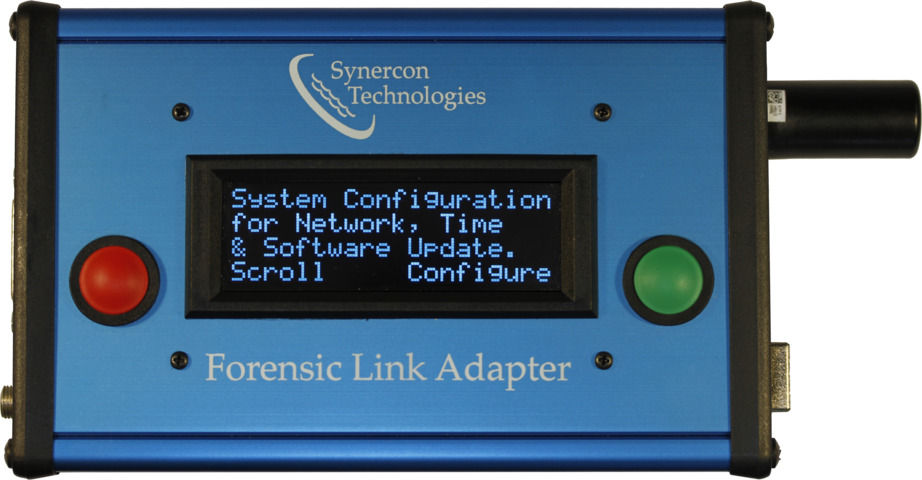
\includegraphics[width=\linewidth]{../media/fla_screens/ethernet_and_others/main/sys_conf}
\end{minipage}
\\[\baselineskip]
\noindent\begin{minipage}{0.45\textwidth}% adapt widths of minipages to your needs
\begin{center}
\textbf{2}\\[\baselineskip]
\end{center}
Enter the configuration sub-menu. This will take you to the Update Software screen.
\end{minipage}%
\hfill%
\begin{minipage}{0.45\textwidth}
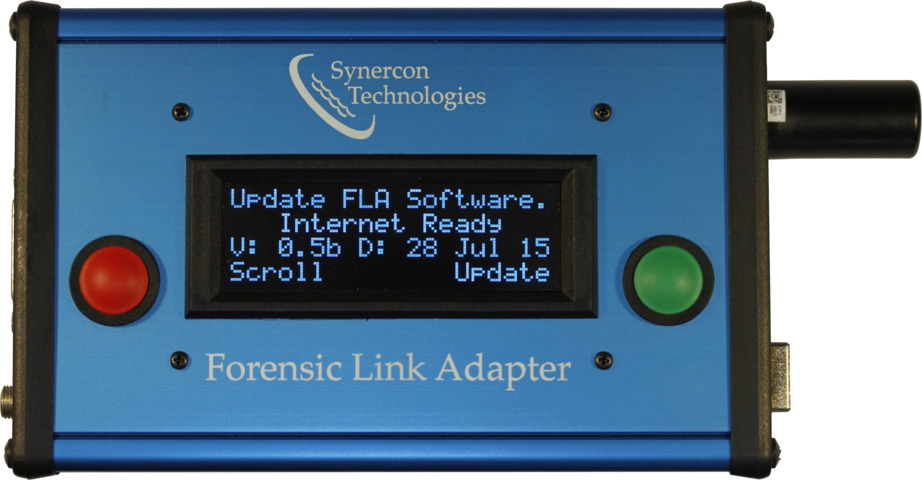
\includegraphics[width=\linewidth]{../media/fla_screens/ethernet_and_others/sys_conf/update_software}
\end{minipage}
\\[\baselineskip]
From this screen, select update. A confirmation screen will appear to prevent accidental updates.\newline
After the update completes, the FLA will require a shutdown. Select "Shutdown" to shut the device down before unplugging it. After the devices indicates it is safe to do so, unplug the power supply. After waiting 10 seconds, plug the device in to continue.
\paragraph{  }
If time displayed on the FLA is not correct, the time can be updated through the configuration menu. As with the update, an Internet connection is required. The timezone of the FLA can also be changed in the system configuration menu. For more information about setting the time and timezone, refer to the FLA User Manual.
\section{Download Appropriate Drivers}
\paragraph{  }
The FLA can act as an RP-1210 device for using OEM software. This only required if the ECM being downloaded is not supported. For a list of supported modules, refer to the FLA User Manual. The drivers for the RP-1210 feature of the FLA can be found either at Dearborn Group's website
\url{http://www.dgtech.com/product/dpa/software/DPA4P_136.zip} 
Or on the FLA Preview site.
\paragraph{  }
The FLA Preview site is a website that is generated by the FLA. To access it, first ensure it is powered on, and has an IP address. This can be confirmed by the title screen shown below.
\begin{center}
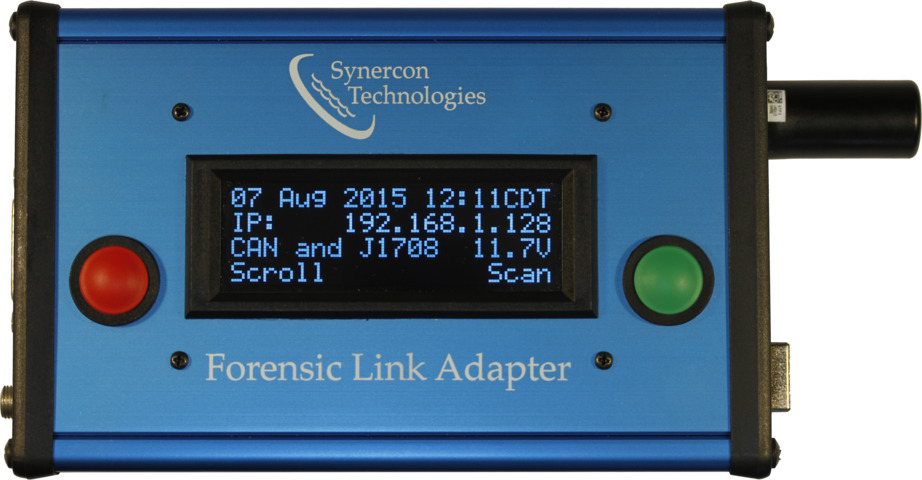
\includegraphics[width=0.5\linewidth]{../media/fla_screens/ethernet_and_others/main/title_both}\label{fig:fla_title_screen}
\end{center}
On a computer connected to the same network, type the IP address into a web browser. The following page should appear.
\begin{center}
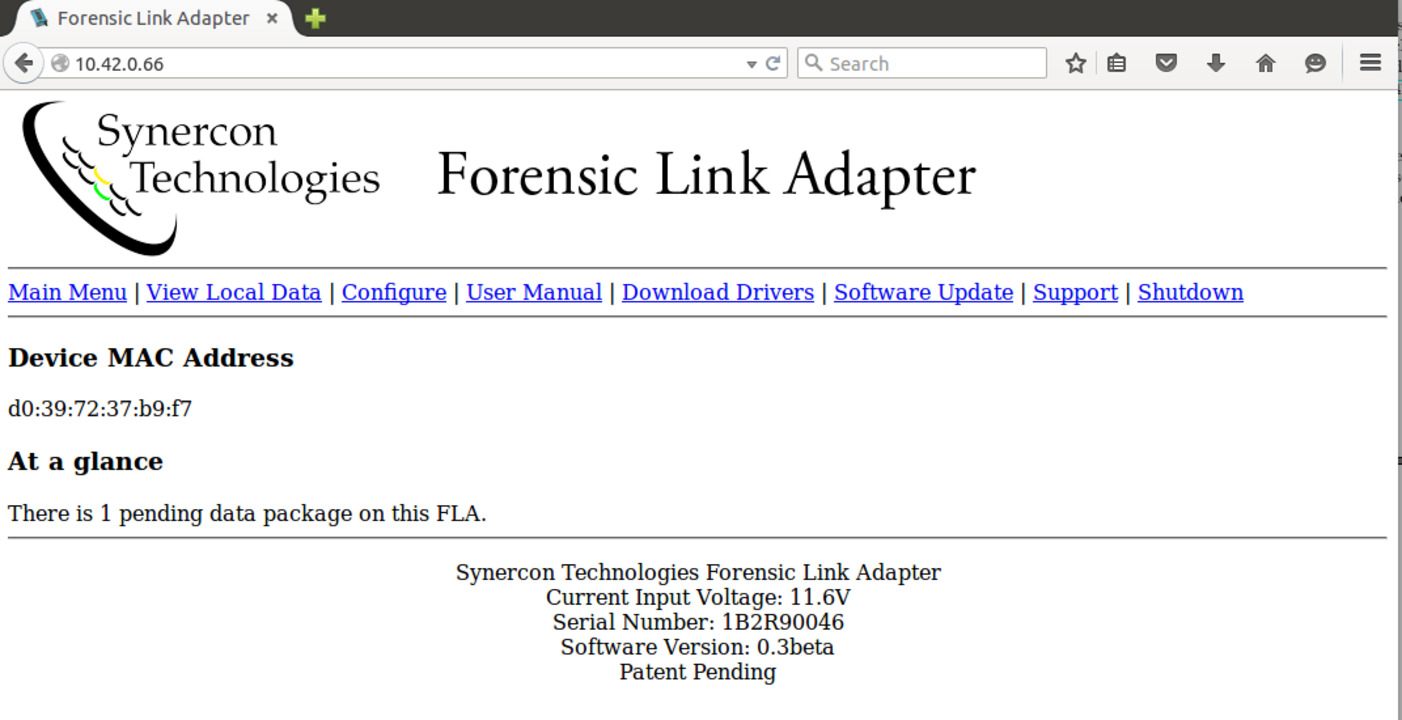
\includegraphics[width=1\linewidth]{../media/fla_preview_screenshots/main_page}\label{fig:preview_main_page}
\end{center}
From this page, select Download Drivers, and then the Download button. The Download Drivers page also has testing instructions to verify RP 1210 is working correctly. This site can be accessed without an Internet connection, as the website is generated by the FLA. For connecting to the site in the field, see section \ref{setting_fla_in_field}.
\section{Manufacturer Software}
If the ECM being downloaded is not supported by the FLA, please ensure a computer has a working copy of the OEM software, and also the RP1210 drivers discussed in the previous section.

\chapter{Setting Up the FLA}
\section{In the Office Use}\label{sec:setting_fla_in_office}
\paragraph{  }
When the FLA is in use at the office, ensure the DHCP server is off. If left on, this can cause problems with the network the FLA is plugged into.
\begin{center}
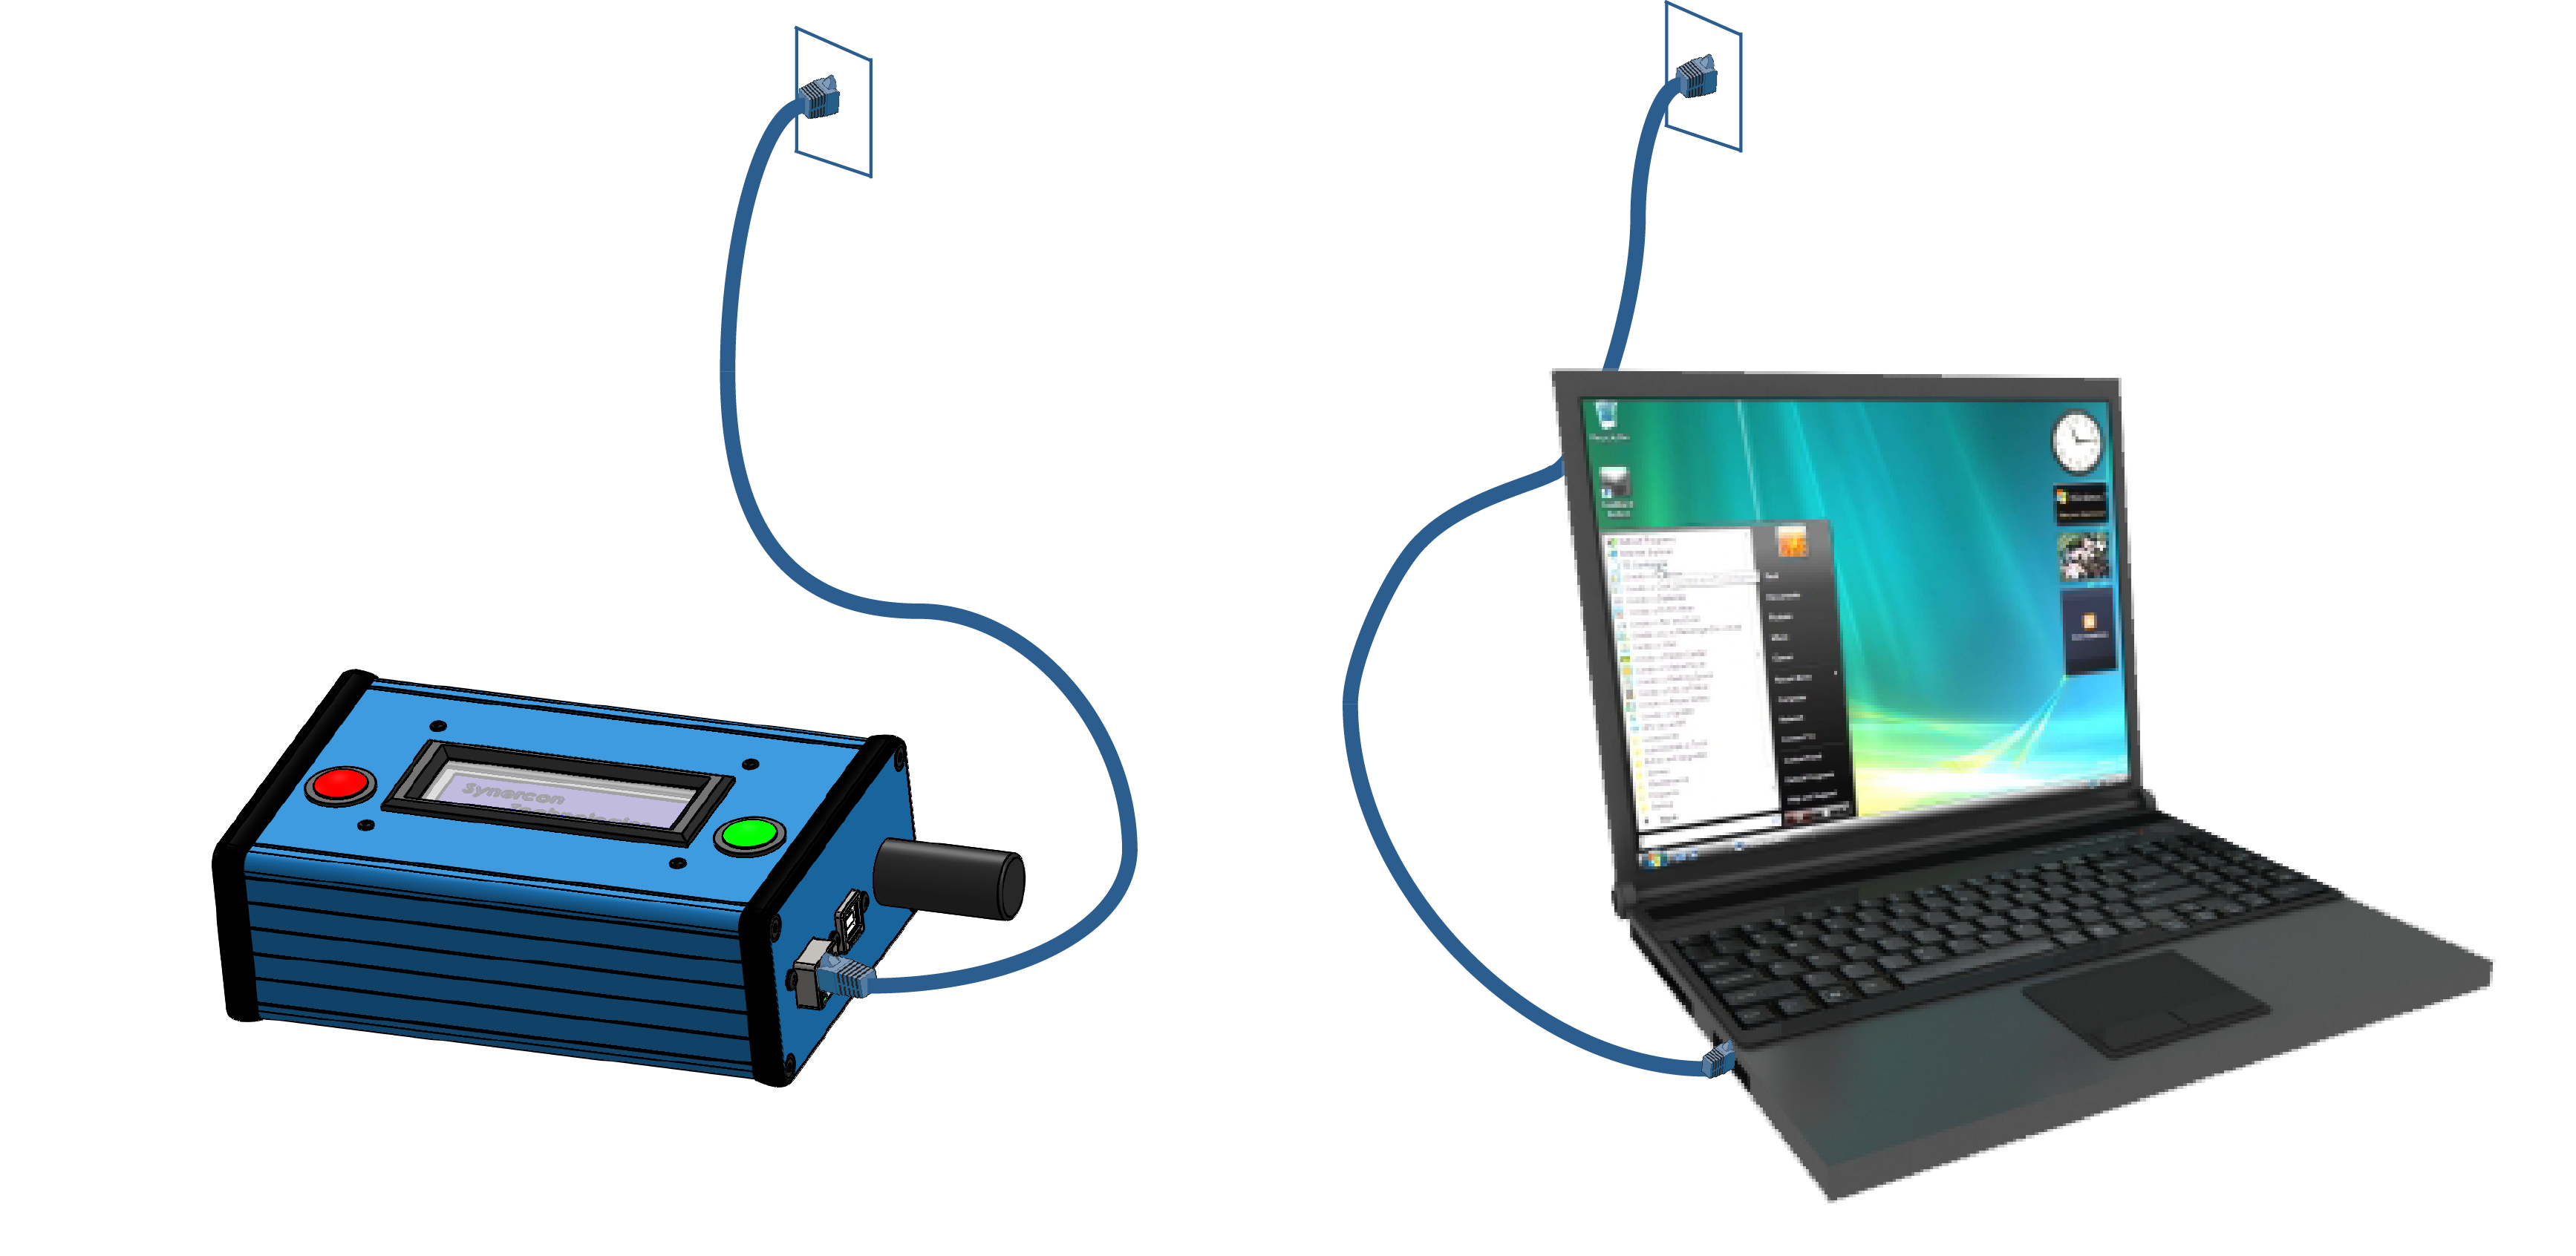
\includegraphics[width=.9\linewidth]{../media/graphics/fla_in_office}
\end{center}
\paragraph{  }
When the FLA is being used with a foreign network, such as any network that is not your home or work network, extra caution must be taken. The local site can be accessed by anyone on the same network, so caution must be taken when using foreign networks. It is not recommended to plug the FLA into an unknown network.
\section{At Home Use}\label{sec:setting_fla_at_home}
\paragraph{  }
When the FLA is in use at a home, or other non-commercial site with an Internet connection, the DHCP server should be turned off. If left on, it can cause problems with the network the FLA is connected to.
\begin{center}
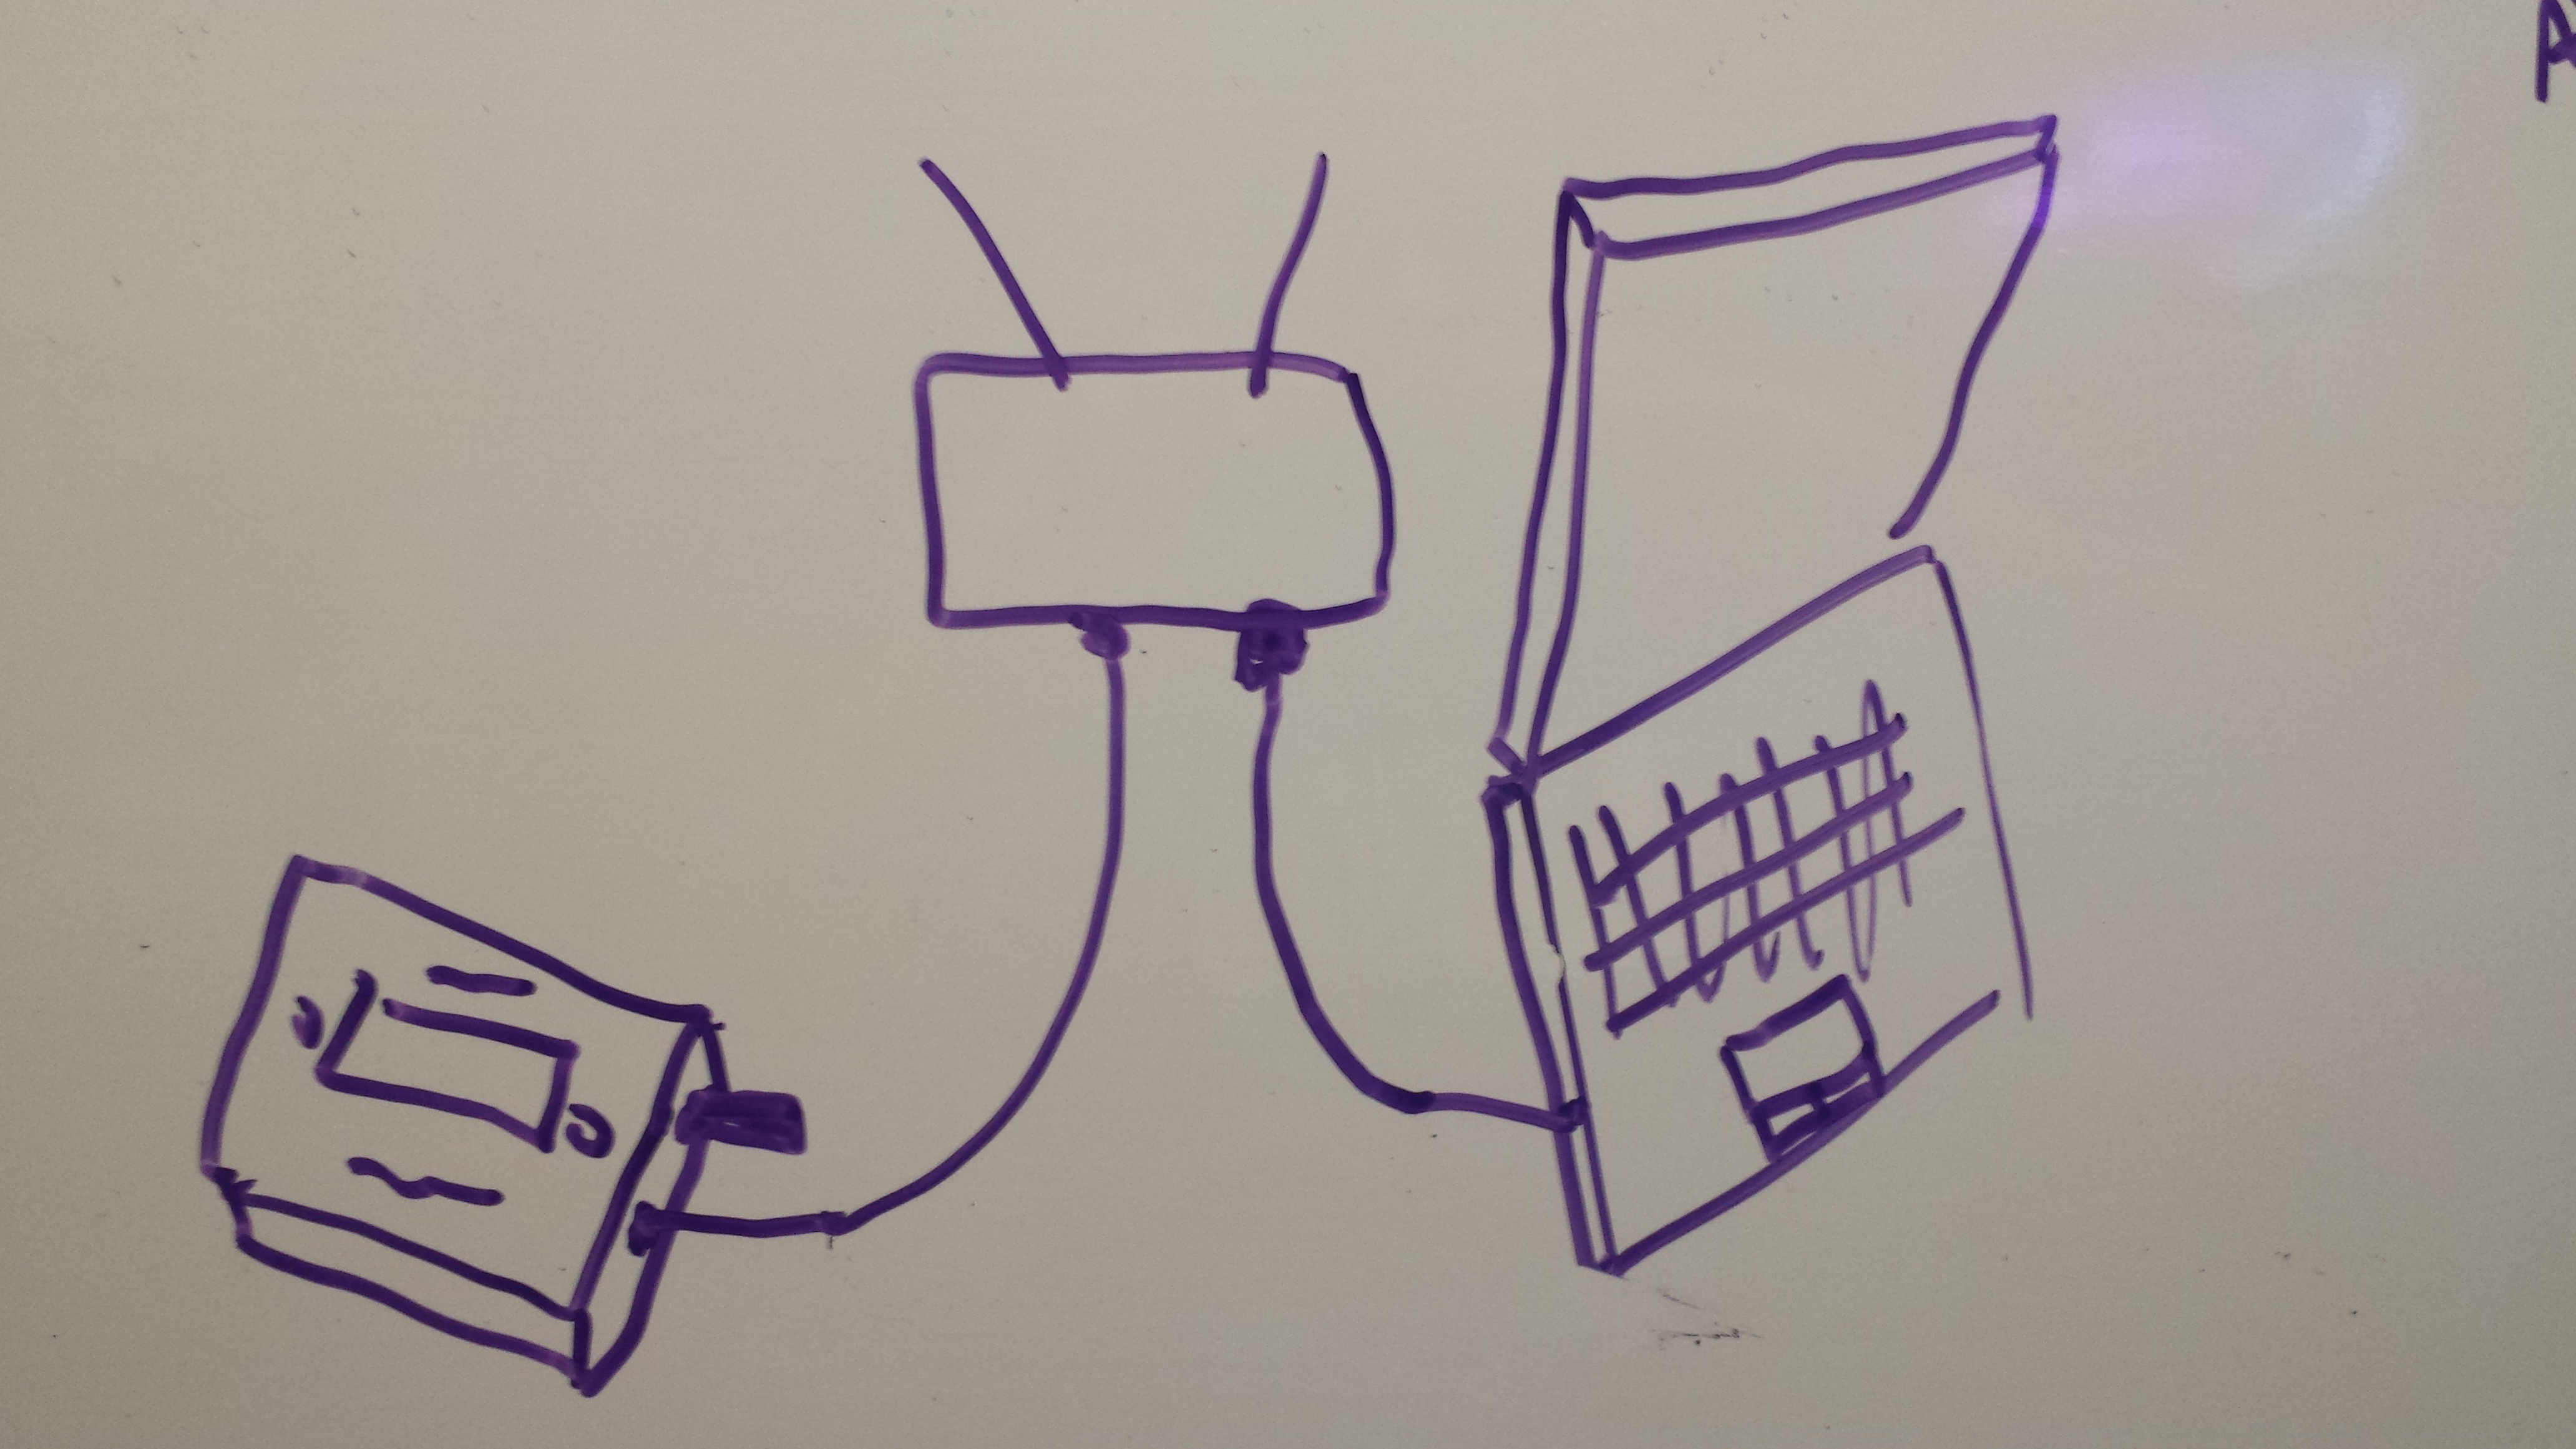
\includegraphics[width=.9\linewidth]{../media/graphics/fla_at_home}
\end{center}
\section{In Field Use}\label{setting_fla_in_field}
\paragraph{  }
When the FLA is being used in the field, the DHCP services may be tuned on. These services allow the user to connect a computer directly to the FLA using the provided Ethernet connection. For more information on DHCP services, refer to section \ref{sec:dhcp_service}.
\begin{center}
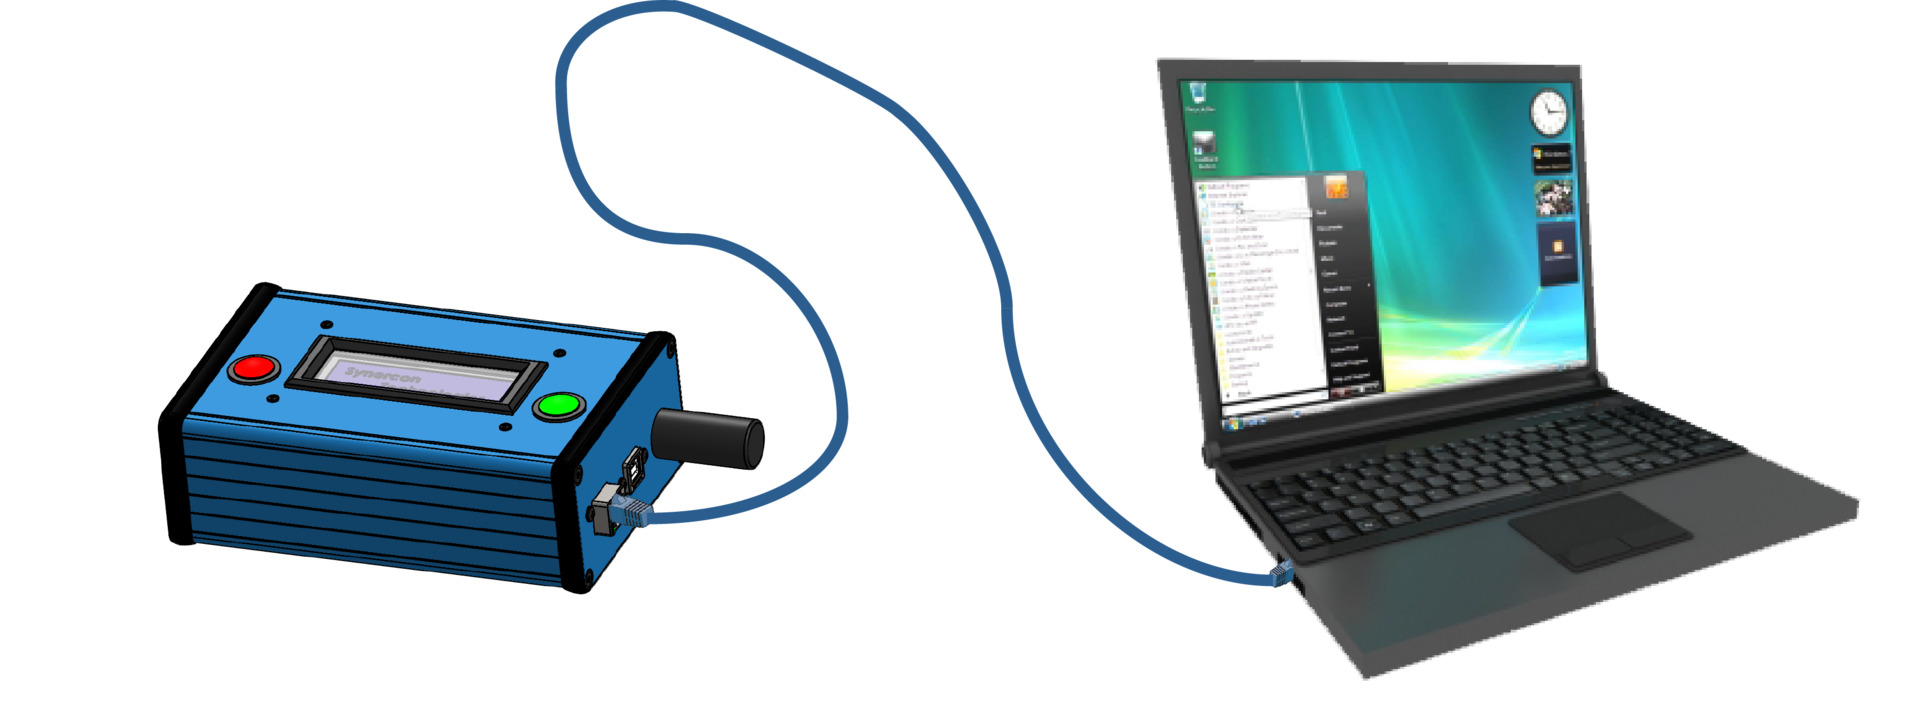
\includegraphics[width=.9\linewidth]{../media/graphics/fla_in_field}
\end{center}
\chapter{Downloading ECMs}
\paragraph{  }
Downloading ECMs will require the FLA, the vehicle to download or the ECMs and a Smart Sensor Simulator, and permission to perform the download.
\\
These are the general steps to perform a download. Some screens may be different depending on the type of ECM being downloaded.
\\[\baselineskip]
\noindent\begin{minipage}{0.45\textwidth}% adapt widths of minipages to your needs
\begin{center}
\textbf{1}\\[\baselineskip]
\end{center}
start at the Title Page and select scan to begin the scan. If the scan option is not present, refer to the troubleshooting section.
\end{minipage}%
\hfill%
\begin{minipage}{0.45\textwidth}
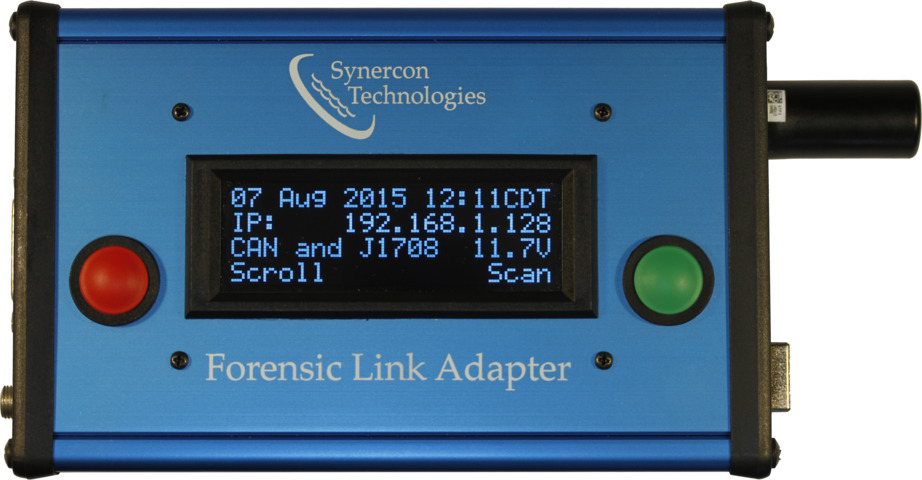
\includegraphics[width=\linewidth]{../media/fla_screens/ethernet_and_others/main/title_both}
\end{minipage}
\\[\baselineskip]\noindent\begin{minipage}{0.45\textwidth}% adapt widths of minipages to your needs
\begin{center}
\textbf{2}\\[\baselineskip]
\end{center}
The device will ask if the operator has sufficient permission to perform the scan and collect data from the vehicle. When the operator continues, this action is time-stamped and rendered with the reports.
\end{minipage}%
\hfill%
\begin{minipage}{0.45\textwidth}
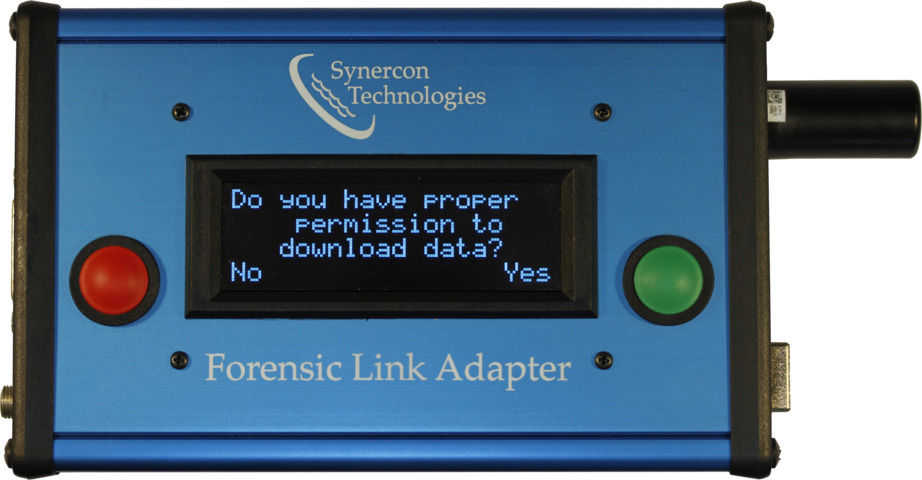
\includegraphics[width=\linewidth]{../media/fla_screens/ethernet_and_others/veh_scan/permission}
\end{minipage}
\\[\baselineskip]

\noindent\begin{minipage}{0.45\textwidth}% adapt widths of minipages to your needs
\begin{center}
\textbf{3}\\[\baselineskip]
\end{center}
The FLA will first listen to the
networks and build a list of all
of the components on the network.
\end{minipage}%
\hfill%
\begin{minipage}{0.45\textwidth}
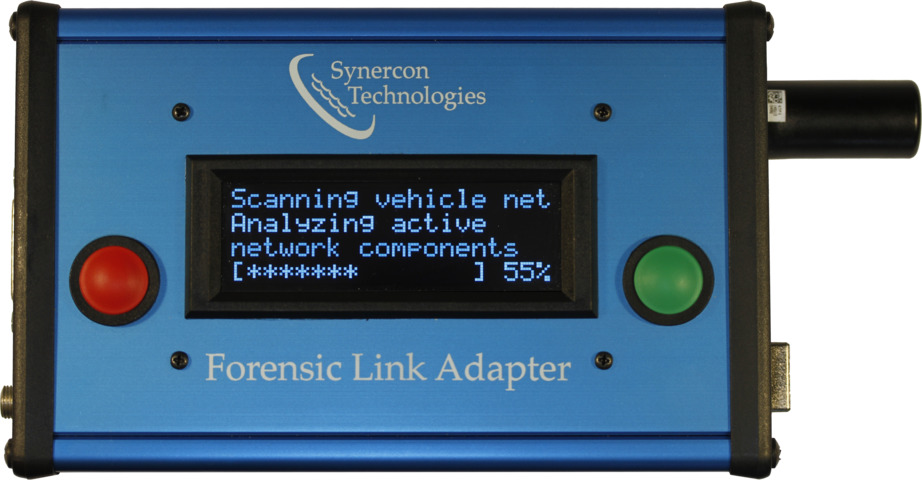
\includegraphics[width=\linewidth]{../media/fla_screens/ethernet_and_others/veh_scan/analyzing_55}
\end{minipage}
\\[\baselineskip]
\noindent\begin{minipage}{0.45\textwidth}% adapt widths of minipages to your needs
\begin{center}
\textbf{4}\\[\baselineskip]
\end{center}
The FLA will then begin the standards-based scan, collecting information such as ECM Component Identification, Mileage, etc.
\end{minipage}%
\hfill%
\begin{minipage}{0.45\textwidth}
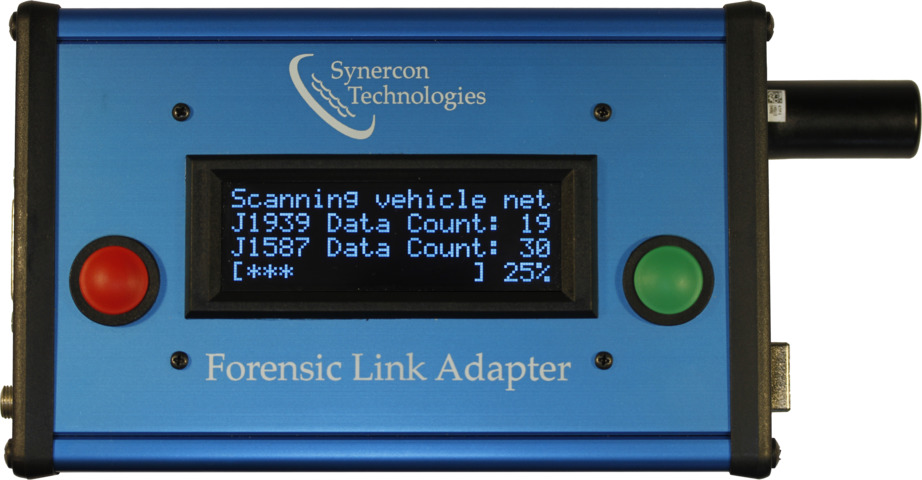
\includegraphics[width=\linewidth]{../media/fla_screens/ethernet_and_others/veh_scan/scan_25}
\end{minipage}
\\[\baselineskip]
\noindent\begin{minipage}{0.45\textwidth}% adapt widths of minipages to your needs
\begin{center}
\textbf{5}\\[\baselineskip]
\end{center}
The FLA will display the Component Id of the engine, as well as the first X characters of the VIN. The full VIN will be in the report. Selecting Continue will continue the scan, Back will cancel the scan.
\end{minipage}%
\hfill%
\begin{minipage}{0.45\textwidth}
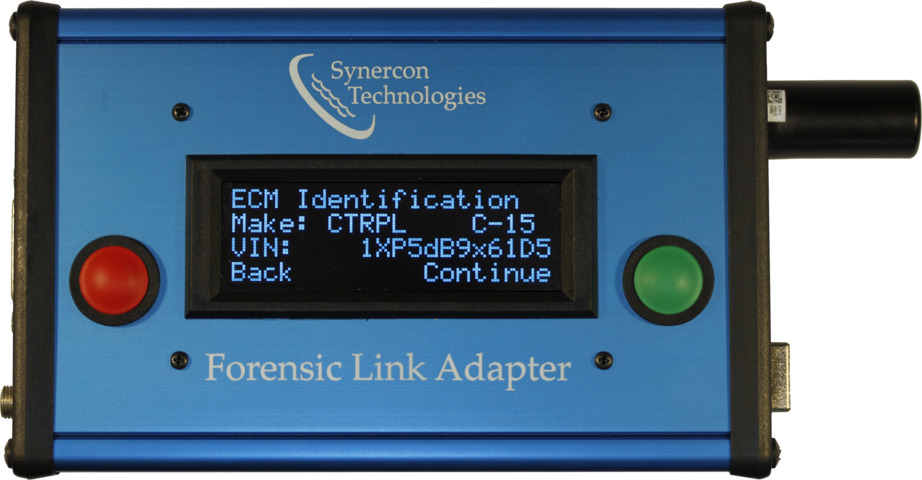
\includegraphics[width=\linewidth]{../media/fla_screens/ethernet_and_others/veh_scan/comp_id}
\end{minipage}
\\[\baselineskip]
\noindent\begin{minipage}{0.45\textwidth}% adapt widths of minipages to your needs
\begin{center}
\textbf{7}\\[\baselineskip]
\end{center}
The FLA will attempt to detect a supported ECM to extract non-standards based data.
\end{minipage}%
\hfill%
\begin{minipage}{0.45\textwidth}
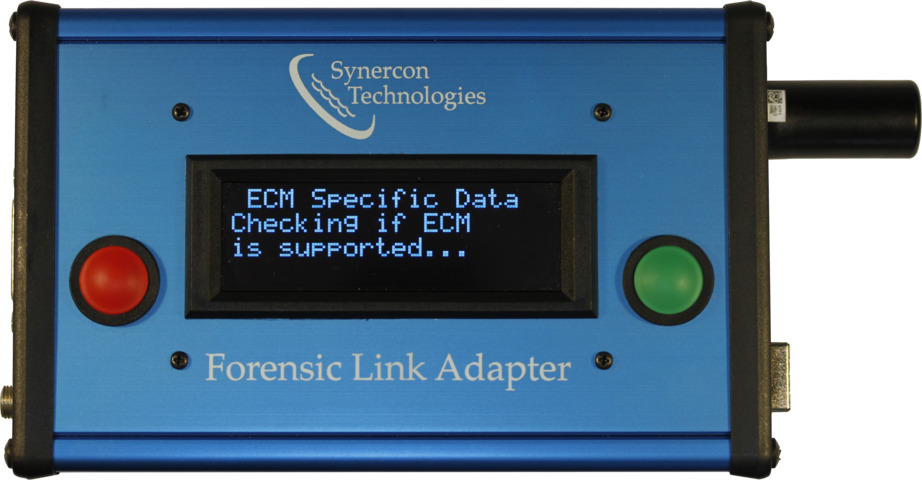
\includegraphics[width=\linewidth]{../media/fla_screens/ethernet_and_others/veh_scan/check_ecm}
\end{minipage}
\\[\baselineskip]
\noindent\begin{minipage}{0.45\textwidth}% adapt widths of minipages to your needs
\begin{center}
\textbf{8.a}\\[\baselineskip]
\end{center}
If the ECM is supported, this screen will ask if the user wishes to collect non-standards based data. See Section X to extract non-standards data with the FLA.
\end{minipage}%
\hfill%
\begin{minipage}{0.45\textwidth}
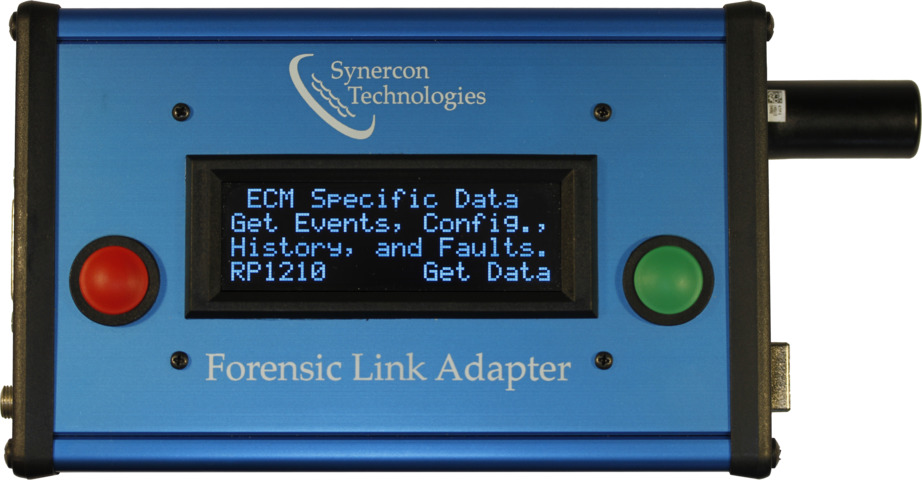
\includegraphics[width=\linewidth]{../media/fla_screens/ethernet_and_others/veh_scan/get_ecm_specific}
\end{minipage}
\\[\baselineskip]
\noindent\begin{minipage}{0.45\textwidth}% adapt widths of minipages to your needs
\begin{center}
\textbf{8.b}\\[\baselineskip]
\end{center}
If the ECM is not supported, please see section X to extract data with OEM software.
\end{minipage}%
\hfill%
\begin{minipage}{0.45\textwidth}
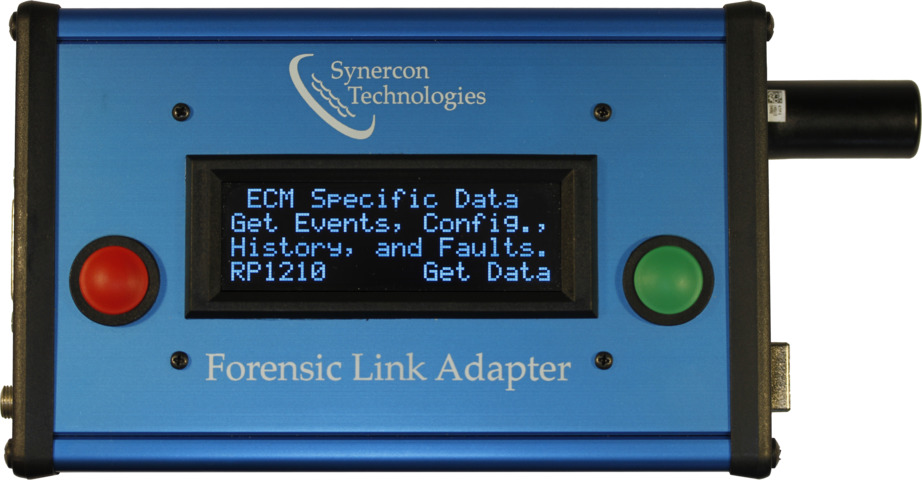
\includegraphics[width=\linewidth]{../media/fla_screens/ethernet_and_others/veh_scan/get_ecm_specific}
\end{minipage}

\section{Supported ECMs}
\paragraph{  }
The FLA can extract more data from supported ECMs, such as event data and other non-standards based data. For a list of supported ECMs, refer to the FLA User Manual. Continuing from screen 8.a from the previous section, select 'Get Data' to continue the non-standards based data extraction. During the extraction, the FLA will display the current status of the extraction. The extraction make take some time, so please wait for the FLA to indicate it is finished. Once completed, the FLA will ask the user if they wish to enable RP1210 mode, or continue to the upload screen. If desired, the FLA can also enable RP1210 mode after performing an extraction. See section~\ref{subsec:upload_data} for more details on uploading data.

\section{Non supported ECMs}
\paragraph{  }
If the FLA is not able to extract data from the ECM, the user can enable RP1210 mode and use the FLA as a passthrough device with the appropriate OEM software.

\chapter{Verifying Data in the Field}
\paragraph{  }
The FLA is able to give the user an overview of the data collected in the field through the FLA Preview. The FLA Preview is a website generated by the FLA that allows the user to connect to the device and examine data on it.
\section{Accessing the FLA Preview}
There are two ways to access the FLA Preview depending on what is available. If a good Ethernet port is available, connect using the at-home/in-office method. If no Ethernet port is available, connect to the preview using the in-field method.
\paragraph{  }
\subsection{At-Home/In-Office}
If the operator is in an office, or at home, they can set the FLA up for home use, section \ref{sec:setting_fla_at_home}, or for office use \ref{sec:setting_fla_in_office}. Enter the IP address from the title screen into a web browser. This will take you to the FLA Preview website. If you have trouble accessing the preview, refer to the troubleshooting section.
\\[\baselineskip]
\noindent\begin{minipage}{0.45\textwidth}% adapt widths of minipages to your needs 
	%\begin{center} 
	%	\textbf{Correct:}\\[\baselineskip] 
	%\end{center} 
	
\includegraphics[width=\linewidth]{../media/fla_preview_screenshots/url_correct} 
\end{minipage}% 
\hfill% 
\begin{minipage}{0.45\textwidth} 
	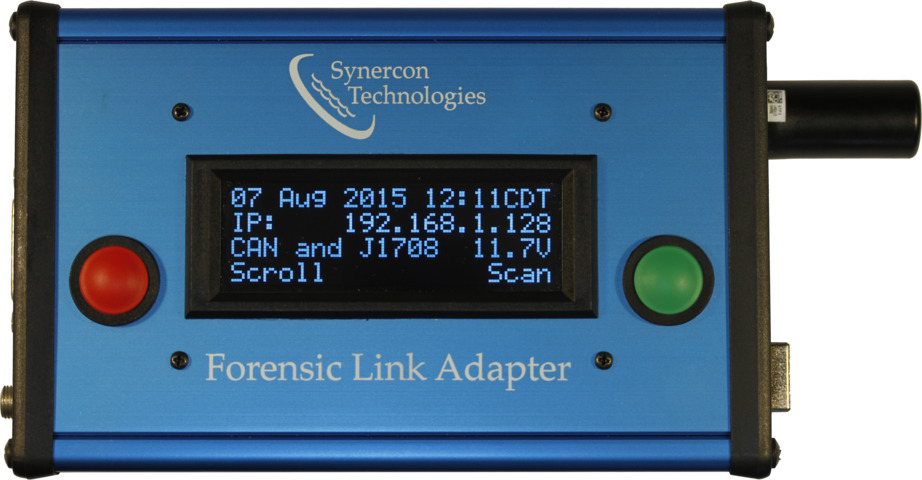
\includegraphics[width=\linewidth]{../media/fla_screens/ethernet_and_others/main/title_both}
\end{minipage}
\subsection{In-Field}
\paragraph{  }
The first step in accessing the FLA Preview is to have the FLA in the correct mode. Unless the operator wishes to place the FLA in support mode, the easiest way to access the FLA Preview is to set up the FLA for the field, as described in section \ref{setting_fla_in_field}. Once the FLA has DHCP enabled, and the computer is directly connected to the FLA with the Ethernet cable, enter "10.0.0.1" into a web browser. This will take you to the FLA Preview website.
\\[\baselineskip]
\noindent\begin{minipage}{0.45\textwidth}% adapt widths of minipages to your needs 
	%\begin{center} 
	%	\textbf{Correct:}\\[\baselineskip] 
	%\end{center} 
	
\includegraphics[width=\linewidth]{../media/fla_preview_screenshots/url_correct_dhcp} 
\end{minipage}% 
\hfill% 
\begin{minipage}{0.45\textwidth} 
	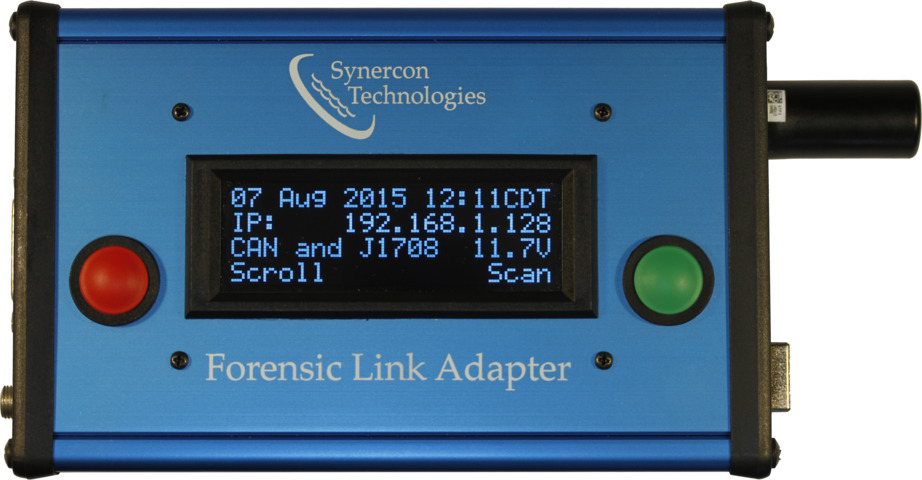
\includegraphics[width=\linewidth]{../media/fla_screens/ethernet_and_others/main/title_both}
\end{minipage}
\section{Using the FLA Preview}
\paragraph{}
The main page of the FLA will show the user how many pending data packages there are on the FLA, as well as if there are any downloads in progress. Under the View Local Data page, the operator can view the data packages that are not yet uploaded to the Synercon Server.
\begin{center}
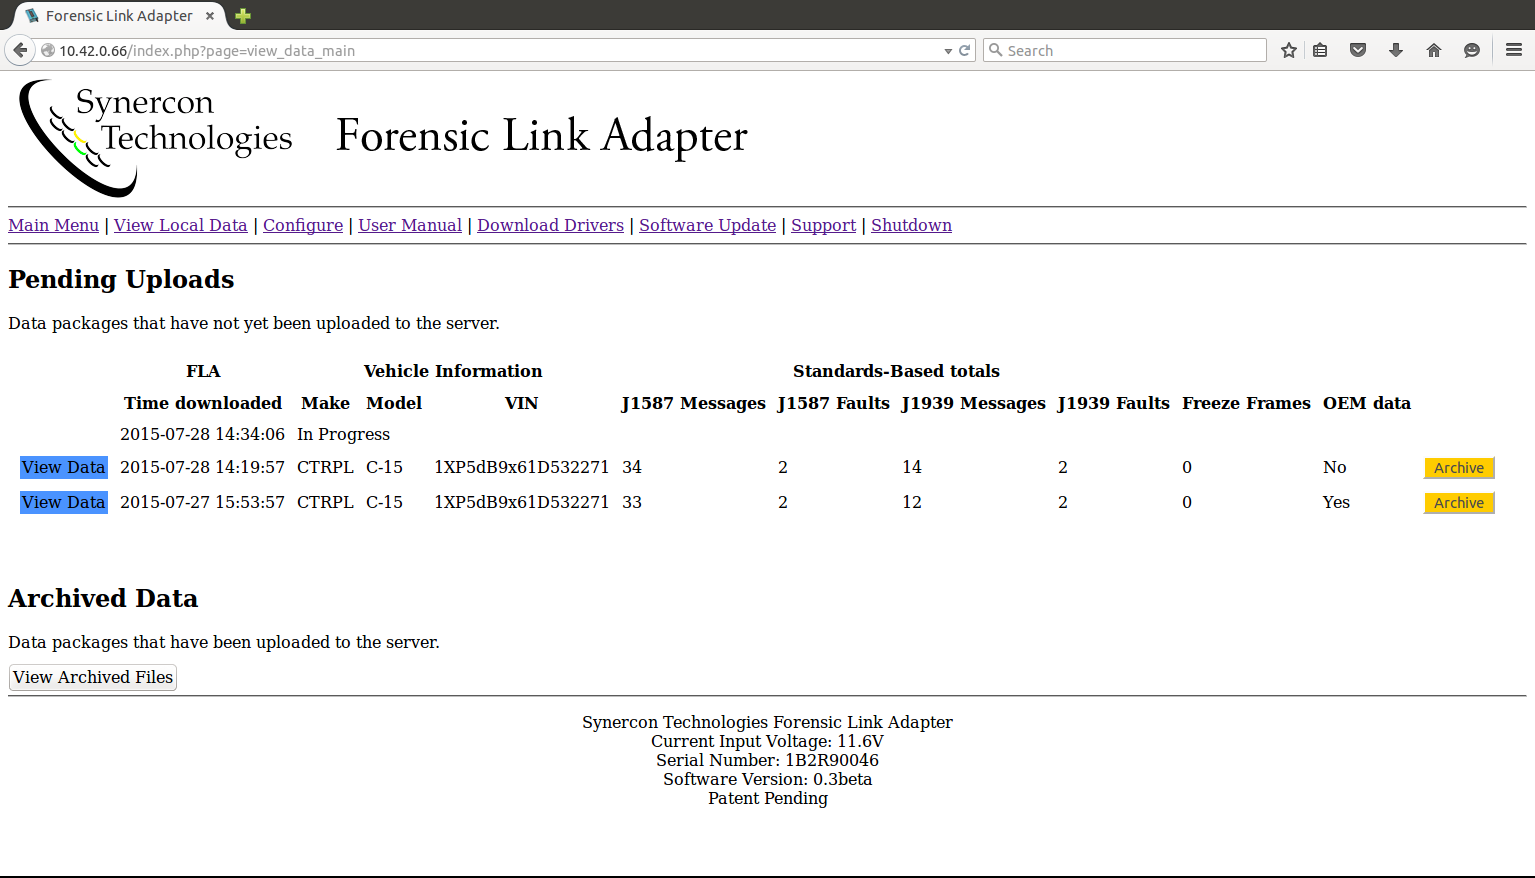
\includegraphics[width=1\linewidth]{../media/fla_preview_screenshots/local_data}
\end{center}
\paragraph{  }
This page gives a brief overview of each data package on the FLA that is not yet uploaded. The OEM data column indicates if the FLA has extracted data from the engine that is not a part of the standards-based extraction. From this page the operator can view the data from an individual data, view archived data packages, or archive pending data packages.
\paragraph{  }
\textbf{Archiving a pending data package will move the data package to the archived list, and it will NOT be uploaded to the server.}
This is only to be used when the operator has a pending data package they do not want to upload on the server, i.e. if it was a practice download, or it contains incomplete data due to a lose cable. Use this with care, archived data packages cannot be un-archived without Synercon support.
\paragraph{  }
The View Data button will allow the operator to view a preview of the report. This will contain all of the standards-based messages, as well as standards-based faults. If the FLA was able to collect non-standards-based data a portion of the decoded data will be available for download. The full records will be available once the operator uploads the data to the Synercon Portal.
\paragraph{  }
The operator can also view archived data with the button at the bottom. Note, the archived page can take some time to load.
\paragraph{  }
\begin{wrapfigure}{r}{0.3\linewidth}
\centering

\includegraphics[width=1\linewidth]{../media/fla_preview_screenshots/download_sha_button}
\end{wrapfigure}
Under each report, the user can download the SHA256 Sums file.
This file contains the SHA 256 sums of all of the files the FLA generated at the time of the download. These sums are cryptographic fingerprints of the files that can be used to determine if the file has changed since the FLA created the file. The user can save this file to perform verification of integrity of data obtained. For more information about SHA256 sums, refer to section~\ref{subsec:using_shas}.

\chapter{Uploading Data to the FLA Portal}
\paragraph{  }
After collecting and verifying data with the FLA, the operator will need to upload the data on the FLA to the FLA Portal to view full reports.
\section{Uploading Data from the FLA}
\label{subsec:upload_data}
\noindent\begin{minipage}{0.45\textwidth}% adapt widths of minipages to your needs
\begin{center}
\textbf{1}\\[\baselineskip]
\end{center}
Ensure the FLA is connected to a working Ethernet port. In the main menu, scroll to the Upload Data screen. Select Upload to initiate the upload.
\end{minipage}%
\hfill%
\begin{minipage}{0.45\textwidth}
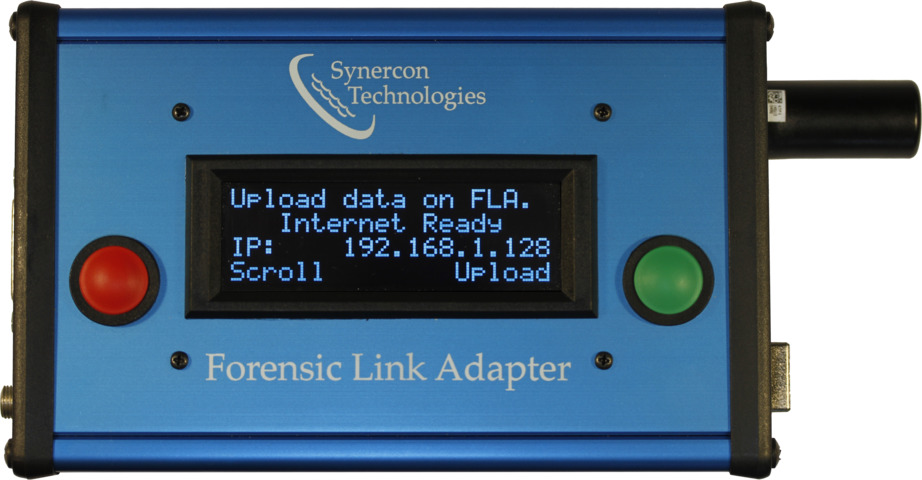
\includegraphics[width=\linewidth]{../media/fla_screens/ethernet_and_others/main/upload_data}
\end{minipage}
\\[\baselineskip]
\noindent\begin{minipage}{0.45\textwidth}% adapt widths of minipages to your needs
\begin{center}
\textbf{2}\\[\baselineskip]
\end{center}
The FLA will connect with the server and will display the number of data packages being uploaded.
\end{minipage}%
\hfill%
\begin{minipage}{0.45\textwidth}
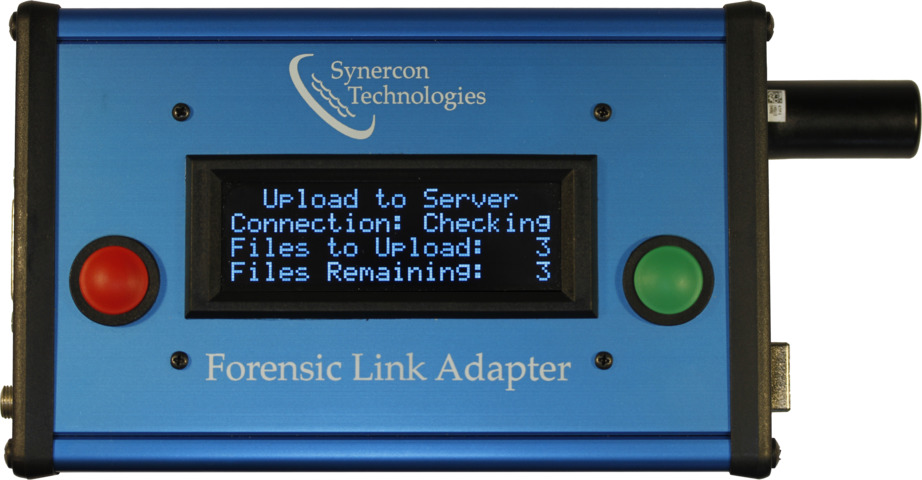
\includegraphics[width=\linewidth]{../media/fla_screens/ethernet_and_others/main/upload_data_checking}
\end{minipage}
\\[\baselineskip]
\noindent\begin{minipage}{0.45\textwidth}% adapt widths of minipages to your needs
\begin{center}
\textbf{3}\\[\baselineskip]
\end{center}
The FLA will then upload the data packages to the Synercon Portal.
\end{minipage}%
\hfill%
\begin{minipage}{0.45\textwidth}
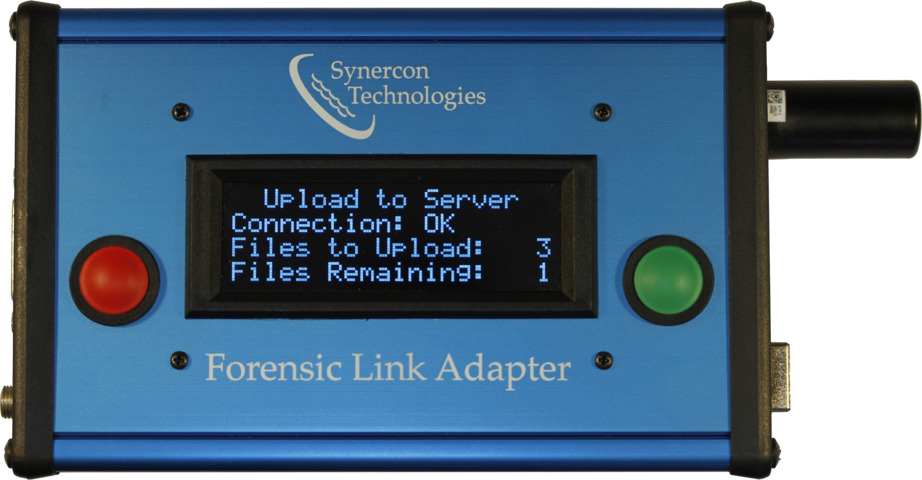
\includegraphics[width=\linewidth]{../media/fla_screens/ethernet_and_others/main/upload_data_in_progress}
\end{minipage}
\\[\baselineskip]
\noindent\begin{minipage}{0.45\textwidth}% adapt widths of minipages to your needs
\begin{center}
\textbf{3}\\[\baselineskip]
\end{center}
When finished, the operator can view the data on the FLA Portal.
\end{minipage}%
\hfill%
\begin{minipage}{0.45\textwidth}
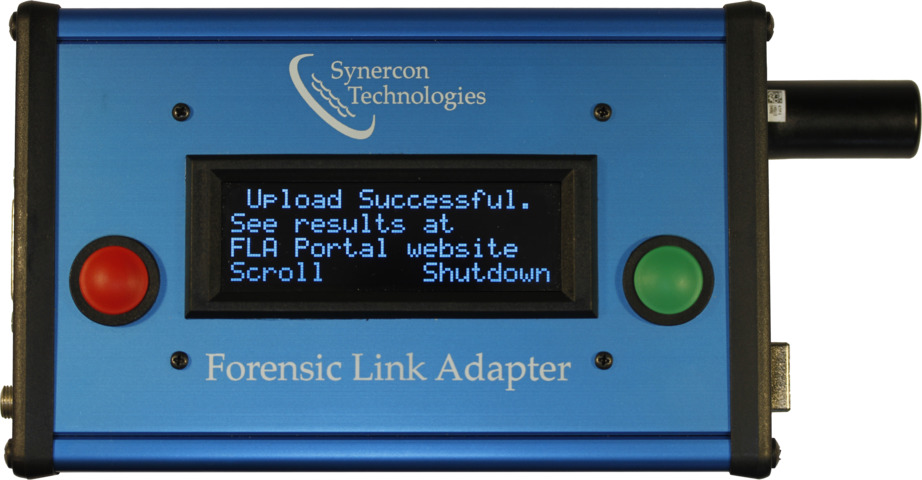
\includegraphics[width=\linewidth]{../media/fla_screens/ethernet_and_others/main/upload_data_complete}
\end{minipage}
\section{Viewing Uploaded Data}
\paragraph{  }
Once the data is uploaded to the FLA Portal, the operator can view the full report. The FLA Portal is viewed by entering \url{fla.synercontechnologies.com} into a web browser.

\chapter{How To}
\paragraph{  }
This section in intended to provide guidance to performing tasks with the FLA. Due to the wide variety of operating systems, web browsers, and configurations of computers, the information and steps in this section are meant as general guidance, and may have to be altered to substituted depending on individual configurations and software on computers used. The operator is advised to consult with any IT or relevant departments or persons before performing any of these steps.
\section{DHCP Services}\label{sec:dhcp_service}
\label{subsec:dhcp_services}
DHCP service is the way devices get IP Addresses on a network in order to communicate with each other. Home and office networks have these services provided, however when out in the field this is not always available. This is where the FLA's DHCP service comes in. When the user wishes to communicate with the FLA, i.e. to preview data on the FLA Preview, they may need to turn on the DHCP services to do so.\\
\textbf{In general, if you plug a computer directly into the FLA using the Ethernet cord, you will need to turn DHCP on. Do not forget to turn it off after you unplug the computer.}
\subsection{Turning DHCP ON}
\noindent\begin{minipage}{0.45\textwidth}% adapt widths of minipages to your needs
\begin{center}
\textbf{1}\\[\baselineskip]
\end{center}
Scroll to the system configuration screen
\end{minipage}%
\hfill%
\begin{minipage}{0.45\textwidth}
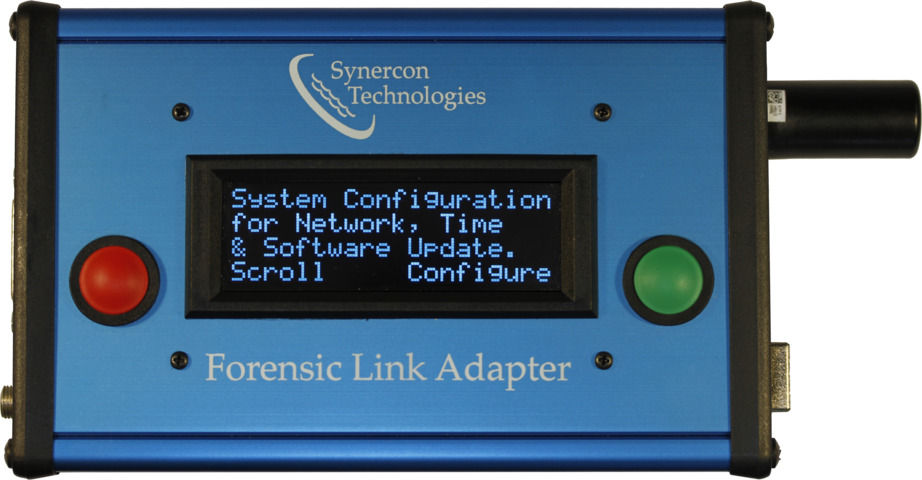
\includegraphics[width=\linewidth]{../media/fla_screens/ethernet_and_others/main/sys_conf}
\end{minipage}
\\[\baselineskip]
\noindent\begin{minipage}{0.45\textwidth}% adapt widths of minipages to your needs
\begin{center}
\textbf{2}\\[\baselineskip]
\end{center}
Scroll to the Change IP Settings screen, and select enable
\end{minipage}%
\hfill%
\begin{minipage}{0.45\textwidth}
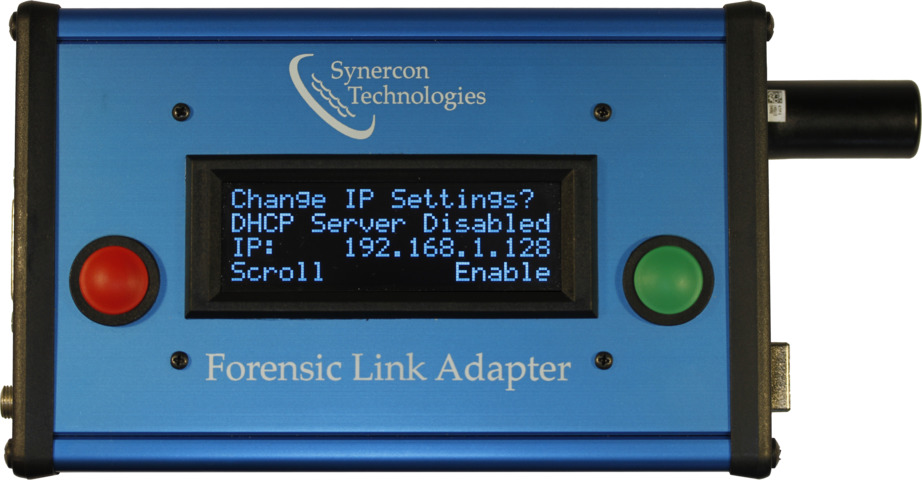
\includegraphics[width=\linewidth]{../media/fla_screens/ethernet_and_others/sys_conf/dhcp_dissabled}
\end{minipage}
\\[\baselineskip]
\noindent\begin{minipage}{0.45\textwidth}% adapt widths of minipages to your needs
\begin{center}
\textbf{3}\\[\baselineskip]
\end{center}
Confirm the request
\end{minipage}%
\hfill%
\begin{minipage}{0.45\textwidth}
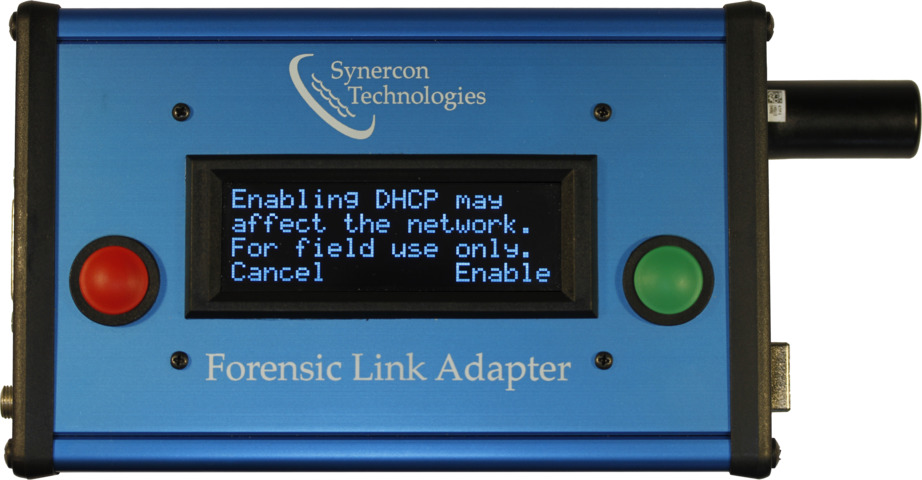
\includegraphics[width=\linewidth]{../media/fla_screens/ethernet_and_others/sys_conf/dhcp_enabling}
\end{minipage}
\subsection{Turning DHCP OFF}
\noindent\begin{minipage}{0.45\textwidth}% adapt widths of minipages to your needs
\begin{center}
\textbf{1}\\[\baselineskip]
\end{center}
Scroll to the system configuration screen
\end{minipage}%
\hfill%
\begin{minipage}{0.45\textwidth}
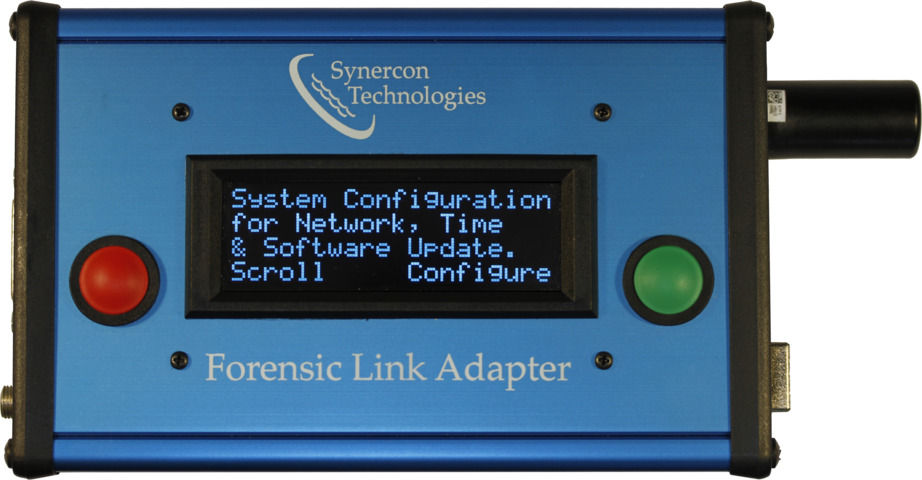
\includegraphics[width=\linewidth]{../media/fla_screens/ethernet_and_others/main/sys_conf}
\end{minipage}
\\[\baselineskip]
\noindent\begin{minipage}{0.45\textwidth}% adapt widths of minipages to your needs
\begin{center}
\textbf{2}\\[\baselineskip]
\end{center}
Scroll to the Change IP Settings screen, and select disable
\end{minipage}%
\hfill%
\begin{minipage}{0.45\textwidth}
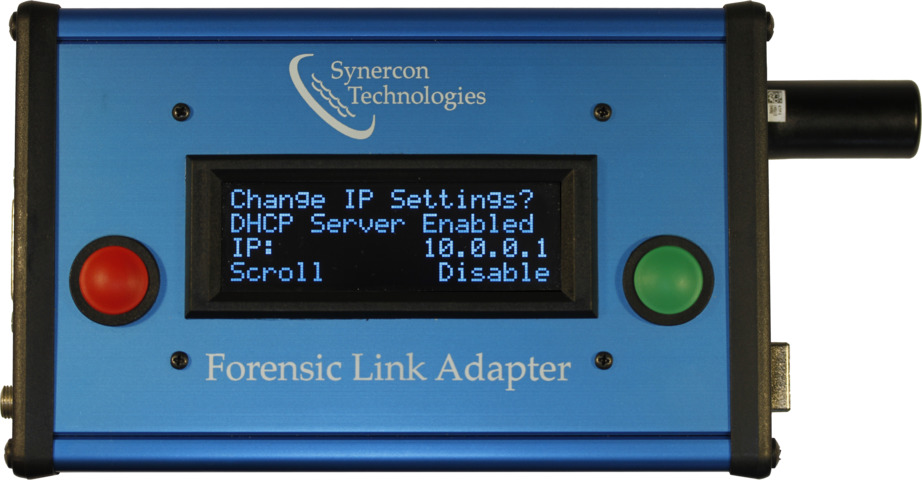
\includegraphics[width=\linewidth]{../media/fla_screens/ethernet_and_others/sys_conf/dhcp_enabled}
\end{minipage}
%\section{Bridge Computer Network}
%\label{subsec:bridge_computer_network}
%This is used for when a secure Ethernet port is not available, however the operator has a computer with a wireless connection to the Internet. This may require administrative privileges. The operator is advised to consult with department IT services before attempting this.
%\subsection{Windows 7}
%\subsection{Windows XP}
%God help you.
\section{Finding the FLA MAC Address}
\label{subsec:finding_mac}
The MAC Address for the FLA is located in the configuration screen.
\\[\baselineskip]
\noindent\begin{minipage}{0.45\textwidth}% adapt widths of minipages to your needs
\begin{center}
\textbf{1}\\[\baselineskip]
\end{center}
Scroll to the system configuration screen, then enter the configuration menu.
\end{minipage}%
\hfill%
\begin{minipage}{0.45\textwidth}
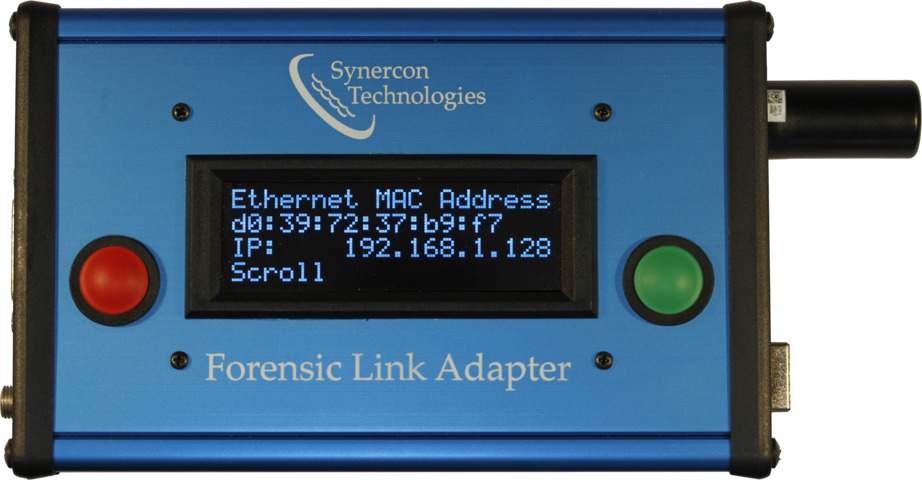
\includegraphics[width=\linewidth]{../media/fla_screens/ethernet_and_others/sys_conf/mac}
\end{minipage}
\\[\baselineskip]
\noindent\begin{minipage}{0.45\textwidth}% adapt widths of minipages to your needs
\begin{center}
\textbf{2}\\[\baselineskip]
\end{center}
Scroll to the Ethernet Mac Address screen. The second line of this screen is the MAC Address. Note, all of the characters are important, so when copying the address, do not forget any of the colons or leading zeros.
\end{minipage}%
\hfill%
\begin{minipage}{0.45\textwidth}
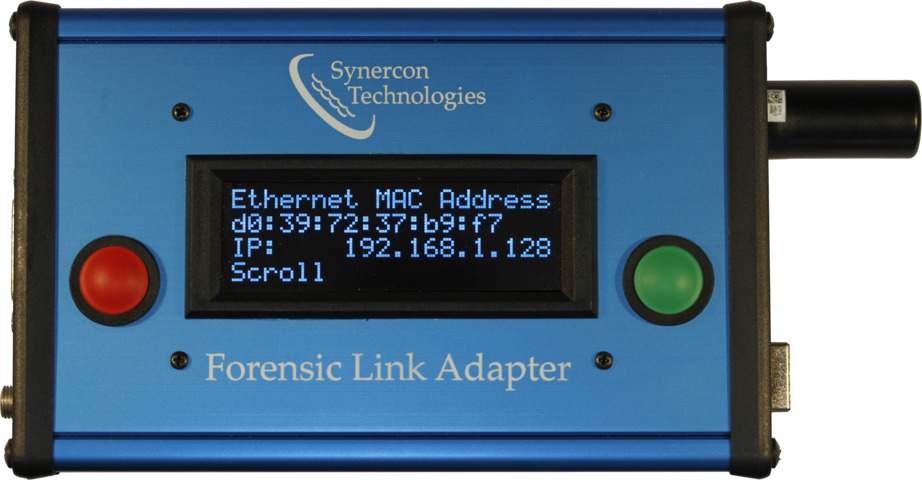
\includegraphics[width=\linewidth]{../media/fla_screens/ethernet_and_others/sys_conf/mac}
\end{minipage}
\\
\section{Using SHA 256 Sums}
\label{subsec:using_shas}
\paragraph{  }
SHA 256 Sums are a cryptographic fingerprint generated on files. Much like a human fingerprint can identify a person, the SHA 256 Sum can identify a file. The FLA will generate SHA 256 Sums for all files used in the download. If any of the data in the files change, the SHA 256 Sum will also change, thus providing a secure way to identify if alterations have been made to data downloaded. When a data package is uploaded to the Synercon Portal, our servers also calculate the SHA 256 Sums for each file, and compare them to the sums the FLA generated. This is done automatically for the user, and the SHA comparisons are shown towards the end of reports on the Synercon Portal. If the user wishes to compare and authenticate the SHAs, the operator can download the SHA 256 Sums file for the report through the FLA Preview, the local website generated by the FLA. This file contains all of the sum strings and the file names. If the user has downloaded any files from the data package, i.e. an XTR report for a DDEC, the user can calculate the SHA 256 Sum of the file and compare the result to the sum listed in the file. Unfortunately Windows does not provide any native program to calculate SHA 256 Sums, the operator would need to download a program to perform the calculations.

\chapter{Troubleshooting}
\section{Do not get the Option to Scan Vehicle}
Symptoms:\\
\noindent\begin{minipage}{0.45\textwidth}% adapt widths of minipages to your needs
The FLA Title Screen does not allow the user to scan the vehicle
\end{minipage}%
\hfill%
\begin{minipage}{0.45\textwidth}
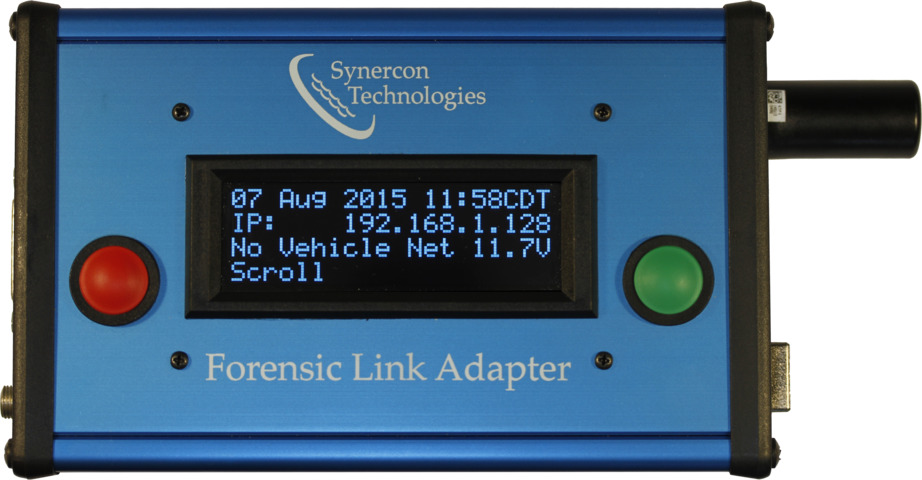
\includegraphics[width=\linewidth]{../media/fla_screens/ethernet_and_others/main/title_no_net}
\end{minipage}\\
Solution:\\
\begin{itemize}
\item Check that the key is in the ON position, with the engine not running.
\item Check to see if the vehicle voltage is nominal, low voltage may prevent ECMs from responding.
\item Check all cables for secure connections.
\end{itemize}
If the above list does not solve the issue, the communication wires from the ECM to the diagnostic port may be damaged. If this is the case, the ECM modules may have to be removed and the operator may have to perform a bench download on the unit. The recommended practice is to use a Synercon Smart Sensor Simulator with the truck ECMs in order to help preserve the data on the modules.

\section{Cannot access the FLA Preview website}
Symptom:\\
The operator is not able to access the FLA Preview website.
Solution:\\
\begin{itemize}
\item navigate to the title screen and verify the FLA has an IP address. If the IP line reads 'cable unplugged', or 'finding IP address', see the FLA Does not have an IP Address section.
\item If the FLA is not connected directly to a computer (i.e. the FLA is plugged into an Ethernet port in an office, or home) ensure the DHCP service is off. If the IP address of the FLA is 10.0.0.1, the DHCP service is likely on. For more information about the DHCP service, see section~\ref{subsec:dhcp_services}.
\item Ensure the operator has typed in the IP address exactly as it appears on the FLA, do not add any extra characters, such as leading zeros before the numbers, or extra spaces.
\end{itemize}
\noindent\begin{minipage}{0.45\textwidth}% adapt widths of minipages to your needs
\begin{center}
\textbf{Correct:}\\[\baselineskip]
\end{center}

\includegraphics[width=\linewidth]{../media/fla_preview_screenshots/url_correct}
\begin{center}
\textbf{Incorrect:}\\[\baselineskip]
\end{center}

\includegraphics[width=\linewidth]{../media/fla_preview_screenshots/url_wrong_1}
\\[0.5\baselineskip]
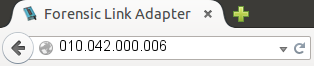
\includegraphics[width=\linewidth]{../media/fla_preview_screenshots/url_wrong_2}
\\[0.5\baselineskip]

\includegraphics[width=\linewidth]{../media/fla_preview_screenshots/url_wrong_3}
\end{minipage}%
\hfill%
\begin{minipage}{0.45\textwidth}
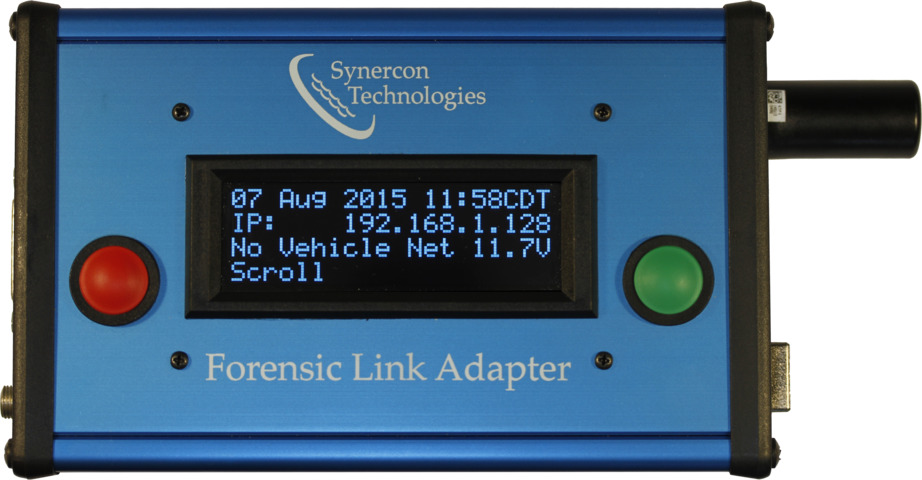
\includegraphics[width=\linewidth]{../media/fla_screens/ethernet_and_others/main/title_no_net}
\end{minipage}
\begin{itemize}
\item Ensure the FLA is on the same network as the computer used to access it. Depending on the configuration, if the computer is connected to a wireless network, try to plug into an Ethernet cable near the port the FLA is plugged into.
\end{itemize}
If the above steps do not resolve the problem, the operator may need to contact the department IT services. If they are not able to resolve the issue, please contact Synercon support.

\section{FLA Does not Have an IP Address}
\subsection{IP says Ethernet Unplugged}
Symptom:\\
\noindent\begin{minipage}{0.45\textwidth}% adapt widths of minipages to your needs
The IP line of the FLA Title screen says Ethernet Unplugged
\end{minipage}%
\hfill%
\begin{minipage}{0.45\textwidth}
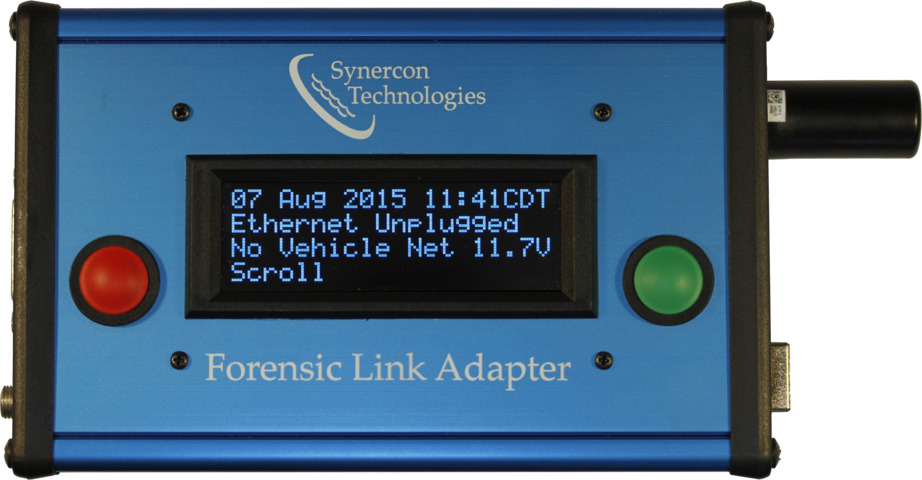
\includegraphics[width=\linewidth]{../media/fla_screens/no_ethernet/title_no_net}
\end{minipage}\\
Solution:\\
\begin{itemize}
\item Check cables are plugged in all the way.
\item Reboot the FLA with the Ethernet cable plugged in.
\item Verify the port is working with a computer.
\item Contact your department IT services, and ensure the FLA is given the permissions to access the Internet. Often this is done by 'whitelisting a MAC address'. If the operator needs to provide the MAC of the FLA, this can be accessed via the configuration menu. For more information, see section~\ref{subsec:finding_mac}.
\end{itemize}
If the above steps do not solve the issue, the operator may need to contact Synercon support.
\subsection{IP says Finding IP Address}
Symptom:\\
\noindent\begin{minipage}{0.45\textwidth}% adapt widths of minipages to your needs
The IP line of the FLA Title screen says Ethernet Unplugged
\end{minipage}%
\hfill%
\begin{minipage}{0.45\textwidth}
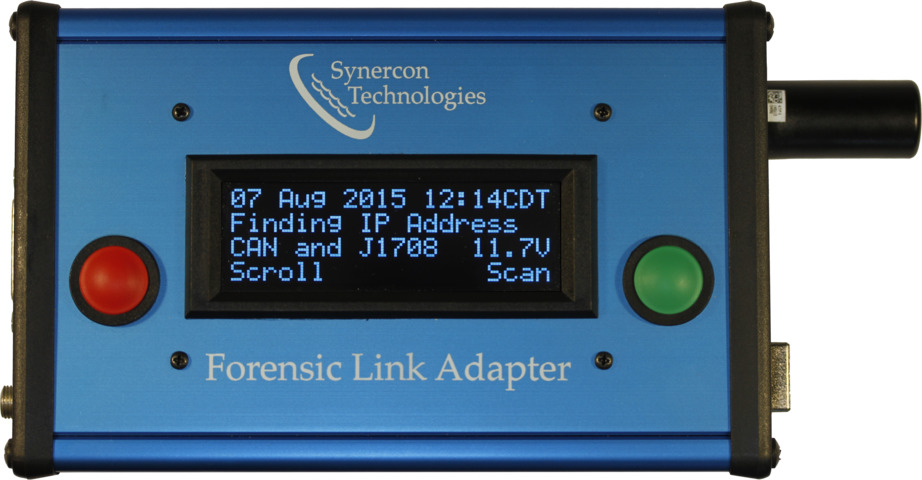
\includegraphics[width=\linewidth]{../media/fla_screens/no_ethernet/title_both_finding_ip}
\end{minipage}\\
Solution:\\
\begin{itemize}
\item If the FLA is being used in the field, and directly connected to a computer, enable the DHCP service. See section~\ref{subsec:dhcp_services}.
\item Reboot the FLA with the Ethernet cable plugged in.
\item Verify the port is working with a computer.
\item Contact your department IT services, and ensure the FLA is given the permissions to access the Internet. Often this is done by 'whitelisting a MAC address'. If the operator needs to provide the MAC of the FLA, this can be accessed via the configuration menu. For more information, see section~\ref{subsec:finding_mac}.
\end{itemize}
\section{FLA Does not Boot When Plugged in}
Symptom:\\
The FLA does nothing when plugged into a vehicle.
Solution:\\
\begin{itemize}
\item The power wires to the diagnostic port may have been damaged, use the cigarette lighter adapter in the FLA case to provide power to the FLA. It is recommended to carry a portable battery for powering the FLA via battery for such situations.
\end{itemize}
If the FLA will not boot with either the cigarette lighter adapter plugged into a know charged battery, or the wall adapter, please contact Synercon support.
\section{FLA Does not finish booting}
Symptom:\\
\noindent\begin{minipage}{0.45\textwidth}% adapt widths of minipages to your needs
The FLA reaches this screen, and does not proceed to the Title screen for more than 30 seconds.
\end{minipage}%
\hfill%
\begin{minipage}{0.45\textwidth}
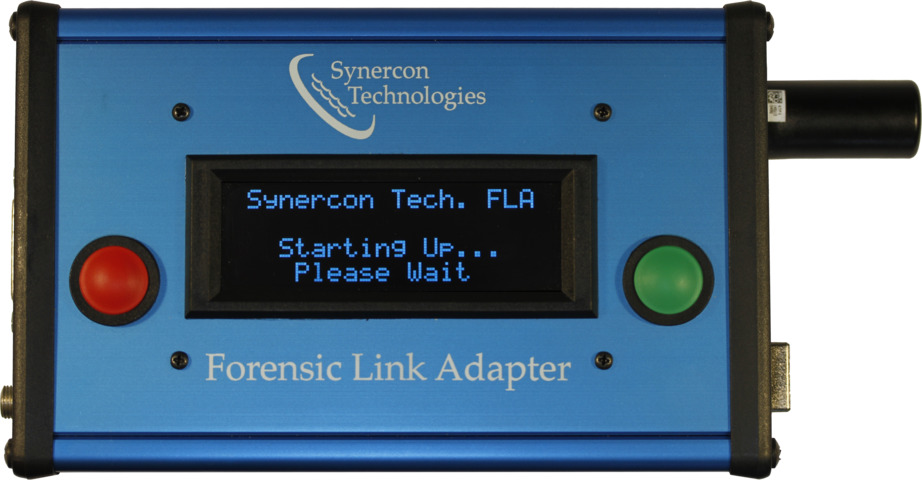
\includegraphics[width=\linewidth]{../media/fla_screens/ethernet_and_others/boot/please_wait}
\end{minipage}\\
Solution:\\
\begin{itemize}
\item Wait 30 seconds for the system to attempt to boot.
\item If the system does not boot, remove power sources, wait 30 seconds and then plug the FLA in. Note this is not recommended as a standard method to shut the FLA down, only do this when you have exhausted all other methods to shut the system down safely.
\end{itemize}
If the device continues to fail to boot for more than 2 times, please contact Synercon support.

\end{document}
